\chapter[Variáveis ambientais]{Variáveis Ambientais em Modelagem de Distribuição de Espécies}

\begin{objetivos}
	Ao final desta unidade, o estudante deverá ser capaz de compreender o papel das variáveis ambientais em SDM; reconhecer diferenças entre variáveis climáticas, topográficas, edáficas e índices derivados; acessar bases como WorldClim, CHELSA, EarthEnv, SoilGrids e ENVIREM; compreender resolução espacial, extensão geográfica, CRS, reamostragem, recorte e harmonização de camadas; construir pilhas ambientais reprodutíveis em R; e aplicar esses conceitos a um estudo de caso real com \textit{Dinizia excelsa} no bioma Amazônia.
\end{objetivos}

\section{Introdução às variáveis ambientais em SDM}

As variáveis ambientais constituem a base explicativa da Modelagem de Distribuição de Espécies. Elas representam gradientes climáticos, edáficos, topográficos, hidrológicos ou estruturais usados para caracterizar os locais onde uma espécie ocorre e os locais disponíveis para calibração e projeção do modelo. Assim, a qualidade ecológica de um SDM depende diretamente da coerência entre registros de ocorrência, área de calibração, escala espacial e conjunto de variáveis selecionadas \parencite{guisan2005predicting,elith2009,guisan2017habitat}.

Em modelos correlativos, as variáveis ambientais funcionam como preditoras. Elas são usadas para estimar relações estatísticas entre ocorrência da espécie e condições ambientais observadas. No entanto, essas relações não devem ser interpretadas automaticamente como relações causais. Uma variável pode ser importante porque representa diretamente um processo ecológico, mas também pode atuar apenas como substituta de outro gradiente não medido \parencite{franklin2010,guisan2017habitat}.

\begin{conceito}[title={\faBook\quad Variável ambiental não é necessariamente mecanismo ecológico}]
	Uma variável ambiental representa um gradiente associado à distribuição da espécie. O fato de uma variável apresentar alta importância estatística em um modelo não implica necessariamente relação causal direta. A interpretação ecológica deve considerar a história natural da espécie, a escala espacial, a resolução dos dados, o conjunto de variáveis disponíveis e o conhecimento prévio sobre os processos que limitam sua distribuição.
\end{conceito}

\subsection{Espaço ambiental, resolução e escala}

O espaço ambiental corresponde ao conjunto de condições representadas pelas variáveis ambientais usadas no modelo. Enquanto o espaço geográfico é formado por coordenadas, pixels, polígonos e mapas, o espaço ambiental é formado pelos valores das variáveis associadas a cada local. Dois pontos distantes no mapa podem ser ambientalmente semelhantes, enquanto pontos próximos podem ser muito diferentes ao longo de gradientes de altitude, solo, umidade ou cobertura vegetal.

A resolução espacial define o tamanho da unidade mínima de análise. Em dados raster, corresponde ao tamanho do pixel. A extensão geográfica define a área total considerada. A escala ecológica envolve simultaneamente resolução, extensão, tempo e nível de organização biológica. Em ampla escala, o clima tende a atuar como filtro dominante; em escala regional ou local, solo, relevo, hidrologia, cobertura da terra e microclima podem ser determinantes.

\begin{atencao}[title={\faExclamationTriangle\quad Compatibilidade entre ocorrência e ambiente}]
	A resolução das camadas ambientais precisa ser compatível com a precisão dos registros de ocorrência. Um registro com incerteza espacial de vários quilômetros não deve ser interpretado como representação precisa de um pixel ambiental de poucos metros.
\end{atencao}

\section{WorldClim}

O WorldClim é uma das bases climáticas mais utilizadas em SDM. Ele disponibiliza camadas globais de temperatura, precipitação e variáveis bioclimáticas derivadas, com diferentes resoluções espaciais. As variáveis BIOCLIM sintetizam aspectos médios, extremos e sazonais do clima, sendo amplamente usadas em estudos de nicho ecológico, biogeografia e mudanças climáticas \parencite{fick2017worldclim}.

\begin{conceito}[title={\faBook\quad Variáveis BIOCLIM}]
	As variáveis BIOCLIM são descritores climáticos derivados de temperatura e precipitação mensal. Elas incluem temperatura média anual, sazonalidade térmica, temperatura dos trimestres mais quente e mais frio, precipitação anual, sazonalidade da precipitação e precipitação dos trimestres mais úmido, seco, quente e frio.
\end{conceito}

\section{CHELSA}

O CHELSA é uma base climática global de alta resolução desenvolvida para representar padrões climáticos considerando processos orográficos e atmosféricos. Em regiões montanhosas ou com forte heterogeneidade topográfica, o CHELSA pode representar gradientes de precipitação e temperatura de forma mais adequada que bases interpoladas mais simples \parencite{karger2017chelsa}.

\begin{dica}[title={\faLightbulb\quad WorldClim ou CHELSA?}]
	WorldClim é amplamente usado e de fácil acesso. CHELSA pode ser particularmente útil em regiões montanhosas, áreas com forte variação topográfica ou estudos sensíveis à precipitação orográfica. A escolha deve considerar região, escala, objetivo e consistência com projeções futuras.
\end{dica}

\section{EarthEnv}

O EarthEnv reúne variáveis ambientais globais voltadas à caracterização da heterogeneidade ambiental, incluindo produtos derivados de topografia, clima, cobertura e habitat. Em SDM, variáveis de heterogeneidade podem auxiliar em estudos de endemismo, diversidade beta, refúgios ambientais e diferenciação de habitats \parencite{amatulli2018data}.

\section{ENVIREM}

O ENVIREM amplia o conjunto clássico de variáveis bioclimáticas ao incluir índices derivados com maior interpretação ecofisiológica, como variáveis relacionadas à evapotranspiração potencial, umidade climática, continentalidade e balanço água-energia. Essas variáveis podem melhorar a representação ambiental em modelos de nicho ecológico \parencite{title2018envirem}.

\section{Variáveis topográficas}

Variáveis topográficas derivadas de modelos digitais de elevação podem representar gradientes importantes em SDM. Elevação, declividade, orientação de vertente, rugosidade, índice de posição topográfica e heterogeneidade do relevo influenciam microclima, drenagem, exposição solar, erosão, acúmulo de água e distribuição de habitats \parencite{farr2007srtm}.

Em ampla escala, como no bioma Amazônia, a topografia pode parecer menos variável do que em regiões montanhosas, mas ainda pode representar gradientes associados a drenagem, altitude relativa, áreas de terra firme, várzeas, escarpas, interflúvios e condições hidrológicas locais.

\section{Variáveis edáficas e SoilGrids}

Variáveis edáficas são fundamentais para representar filtros ambientais associados à fertilidade, textura, acidez, capacidade de troca catiônica, retenção de água e disponibilidade de nutrientes. O SoilGrids, desenvolvido pelo ISRIC, fornece predições globais de propriedades do solo em múltiplas profundidades, sendo útil para aplicações regionais e globais em SDM \parencite{poggio2021soilgrids}.

\begin{conceito}[title={\faBook\quad Solo como filtro ecológico}]
	O solo representa um componente relativamente estável da paisagem e pode explicar padrões de distribuição que não são capturados apenas por clima. Em plantas, variáveis como pH, textura, carbono orgânico, argila, areia e capacidade de troca catiônica podem estar fortemente associadas à ocorrência.
\end{conceito}

\section{Harmonização de camadas ambientais}

Bases ambientais frequentemente possuem resoluções, extensões, sistemas de coordenadas e unidades diferentes. Antes de usar essas camadas em SDM, é necessário harmonizá-las. Esse processo envolve recorte, reprojeção, reamostragem, padronização de nomes, remoção de camadas redundantes e construção de uma pilha ambiental consistente.

\begin{atencao}[title={\faExclamationTriangle\quad Harmonização antes da modelagem}]
	Nunca combine diretamente camadas ambientais com resoluções, extensões ou projeções diferentes. A inconsistência espacial entre rasters pode gerar extrações erradas de valores ambientais e comprometer todo o modelo.
\end{atencao}

\section{Estudo de caso real: variáveis ambientais para \textit{Dinizia excelsa}}

Nesta seção, os conceitos apresentados anteriormente são aplicados a um estudo de caso real com \textit{Dinizia excelsa} no bioma Amazônia. Os registros de ocorrência foram previamente compilados, limpos, filtrados espacialmente e rarefeitos na Unidade 2. Agora, esses registros são associados a variáveis ambientais reais, recortadas e harmonizadas para a escala do bioma Amazônia.

O objetivo não é apenas gerar mapas ambientais, mas preparar uma base espacial coerente para as etapas seguintes da apostila: controle de multicolinearidade, seleção de variáveis, ajuste de modelos, avaliação, ensemble, projeções climáticas futuras e reconstruções paleoclimáticas.

\begin{aplicacao}
	No estudo de caso com \textit{Dinizia excelsa}, as variáveis ambientais são tratadas como hipóteses ecológicas sobre os gradientes que podem influenciar a distribuição da espécie. Variáveis climáticas representam filtros energéticos e hídricos; variáveis topográficas representam heterogeneidade do terreno; e variáveis edáficas, quando disponíveis, representam filtros associados ao substrato e à fertilidade.
\end{aplicacao}

\subsection{Variáveis bioclimáticas selecionadas}

Para o estudo de caso, foram preparadas variáveis bioclimáticas derivadas do WorldClim e recortadas para o bioma Amazônia. As variáveis selecionadas representam gradientes de temperatura, precipitação e sazonalidade:

\begin{itemize}
	\item BIO3 -- Isotermalidade;
	\item BIO4 -- Sazonalidade da temperatura;
	\item BIO5 -- Temperatura máxima do mês mais quente;
	\item BIO8 -- Temperatura média do trimestre mais úmido;
	\item BIO12 -- Precipitação anual;
	\item BIO13 -- Precipitação do mês mais úmido;
	\item BIO14 -- Precipitação do mês mais seco;
	\item BIO18 -- Precipitação do trimestre mais quente;
	\item BIO19 -- Precipitação do trimestre mais frio.
\end{itemize}

Essas variáveis são úteis para representar componentes climáticos associados à disponibilidade hídrica, estresse térmico, sazonalidade e extremos ambientais. Em espécies arbóreas tropicais, tais gradientes podem estar associados à sobrevivência, crescimento, regeneração, recrutamento e persistência populacional.

\rscriptfile{scripts/unidade03/01_variaveis_ambientais_dinizia.R}

\begin{figure}[H]
	\centering
	\includegraphics[width=0.98\textwidth]{figuras/unidade03/unidade03_variaveis_bioclimaticas_dinizia.png}
	\caption{Variáveis bioclimáticas selecionadas para o bioma Amazônia com registros finais de \textit{Dinizia excelsa}. Cada painel possui escala própria de cores, permitindo visualizar adequadamente gradientes de temperatura, precipitação e sazonalidade.}
	\label{fig:unidade03_variaveis_bioclimaticas_dinizia}
\end{figure}

\subsection{Variáveis topográficas}

Além das variáveis climáticas, o script prepara variáveis topográficas derivadas de um modelo digital de elevação. Nesta unidade, foram calculadas elevação, declividade e orientação de vertente. Essas camadas são harmonizadas com as variáveis bioclimáticas, garantindo mesma resolução, extensão, máscara espacial e sistema de referência.

\begin{figure}[H]
	\centering
	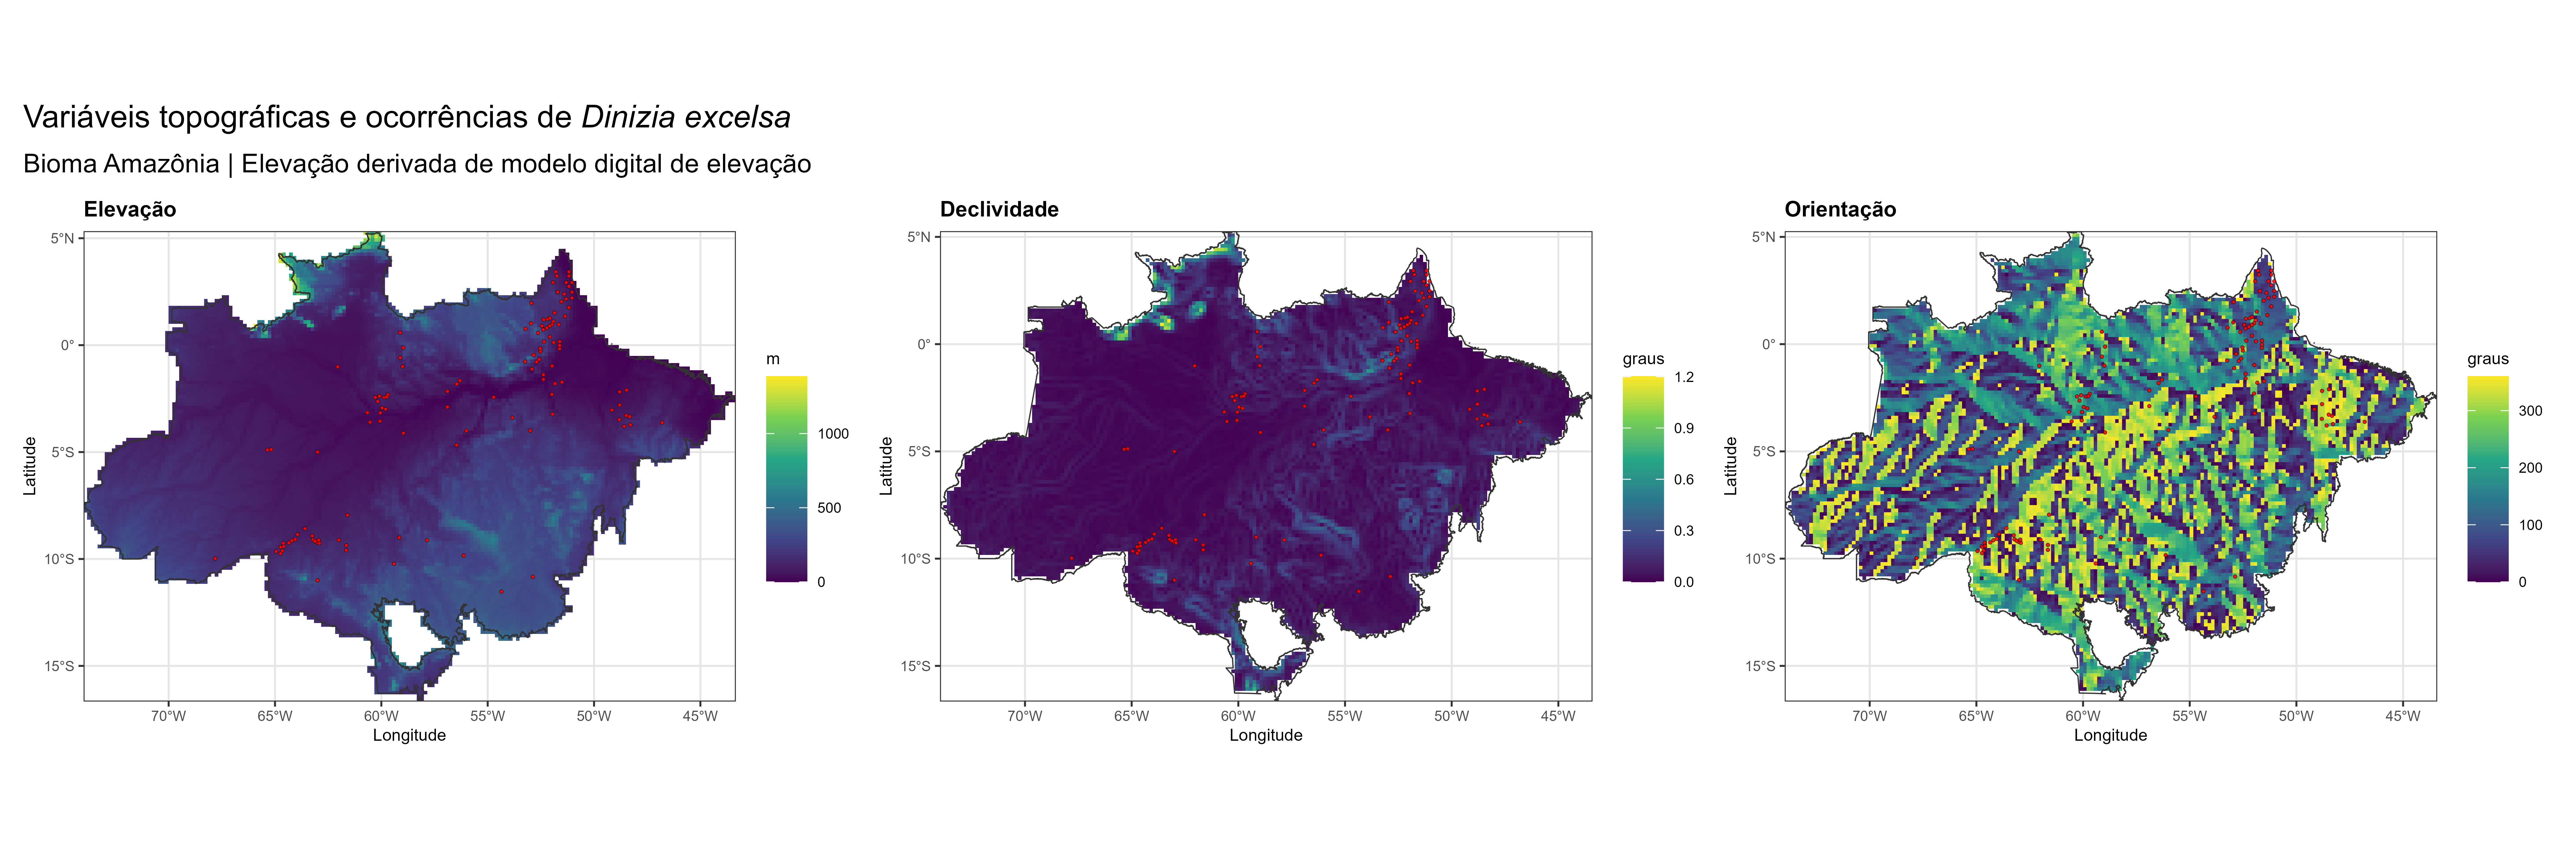
\includegraphics[width=0.98\textwidth]{figuras/unidade03/unidade03_variaveis_topograficas_dinizia.png}
	\caption{Variáveis topográficas preparadas para o bioma Amazônia e associadas ao estudo de caso com \textit{Dinizia excelsa}. Os mapas representam elevação, declividade e orientação de vertente.}
	\label{fig:unidade03_topografia_dinizia}
\end{figure}

\subsection{Extração ambiental nas ocorrências}

Após a preparação das camadas ambientais, os valores de cada variável são extraídos nos pontos finais de ocorrência. Essa matriz ambiental é essencial para as próximas etapas da modelagem, pois permite analisar a amplitude ambiental ocupada pela espécie, avaliar correlações entre variáveis, selecionar preditores e construir modelos de adequabilidade.

\begin{figure}[H]
	\centering
	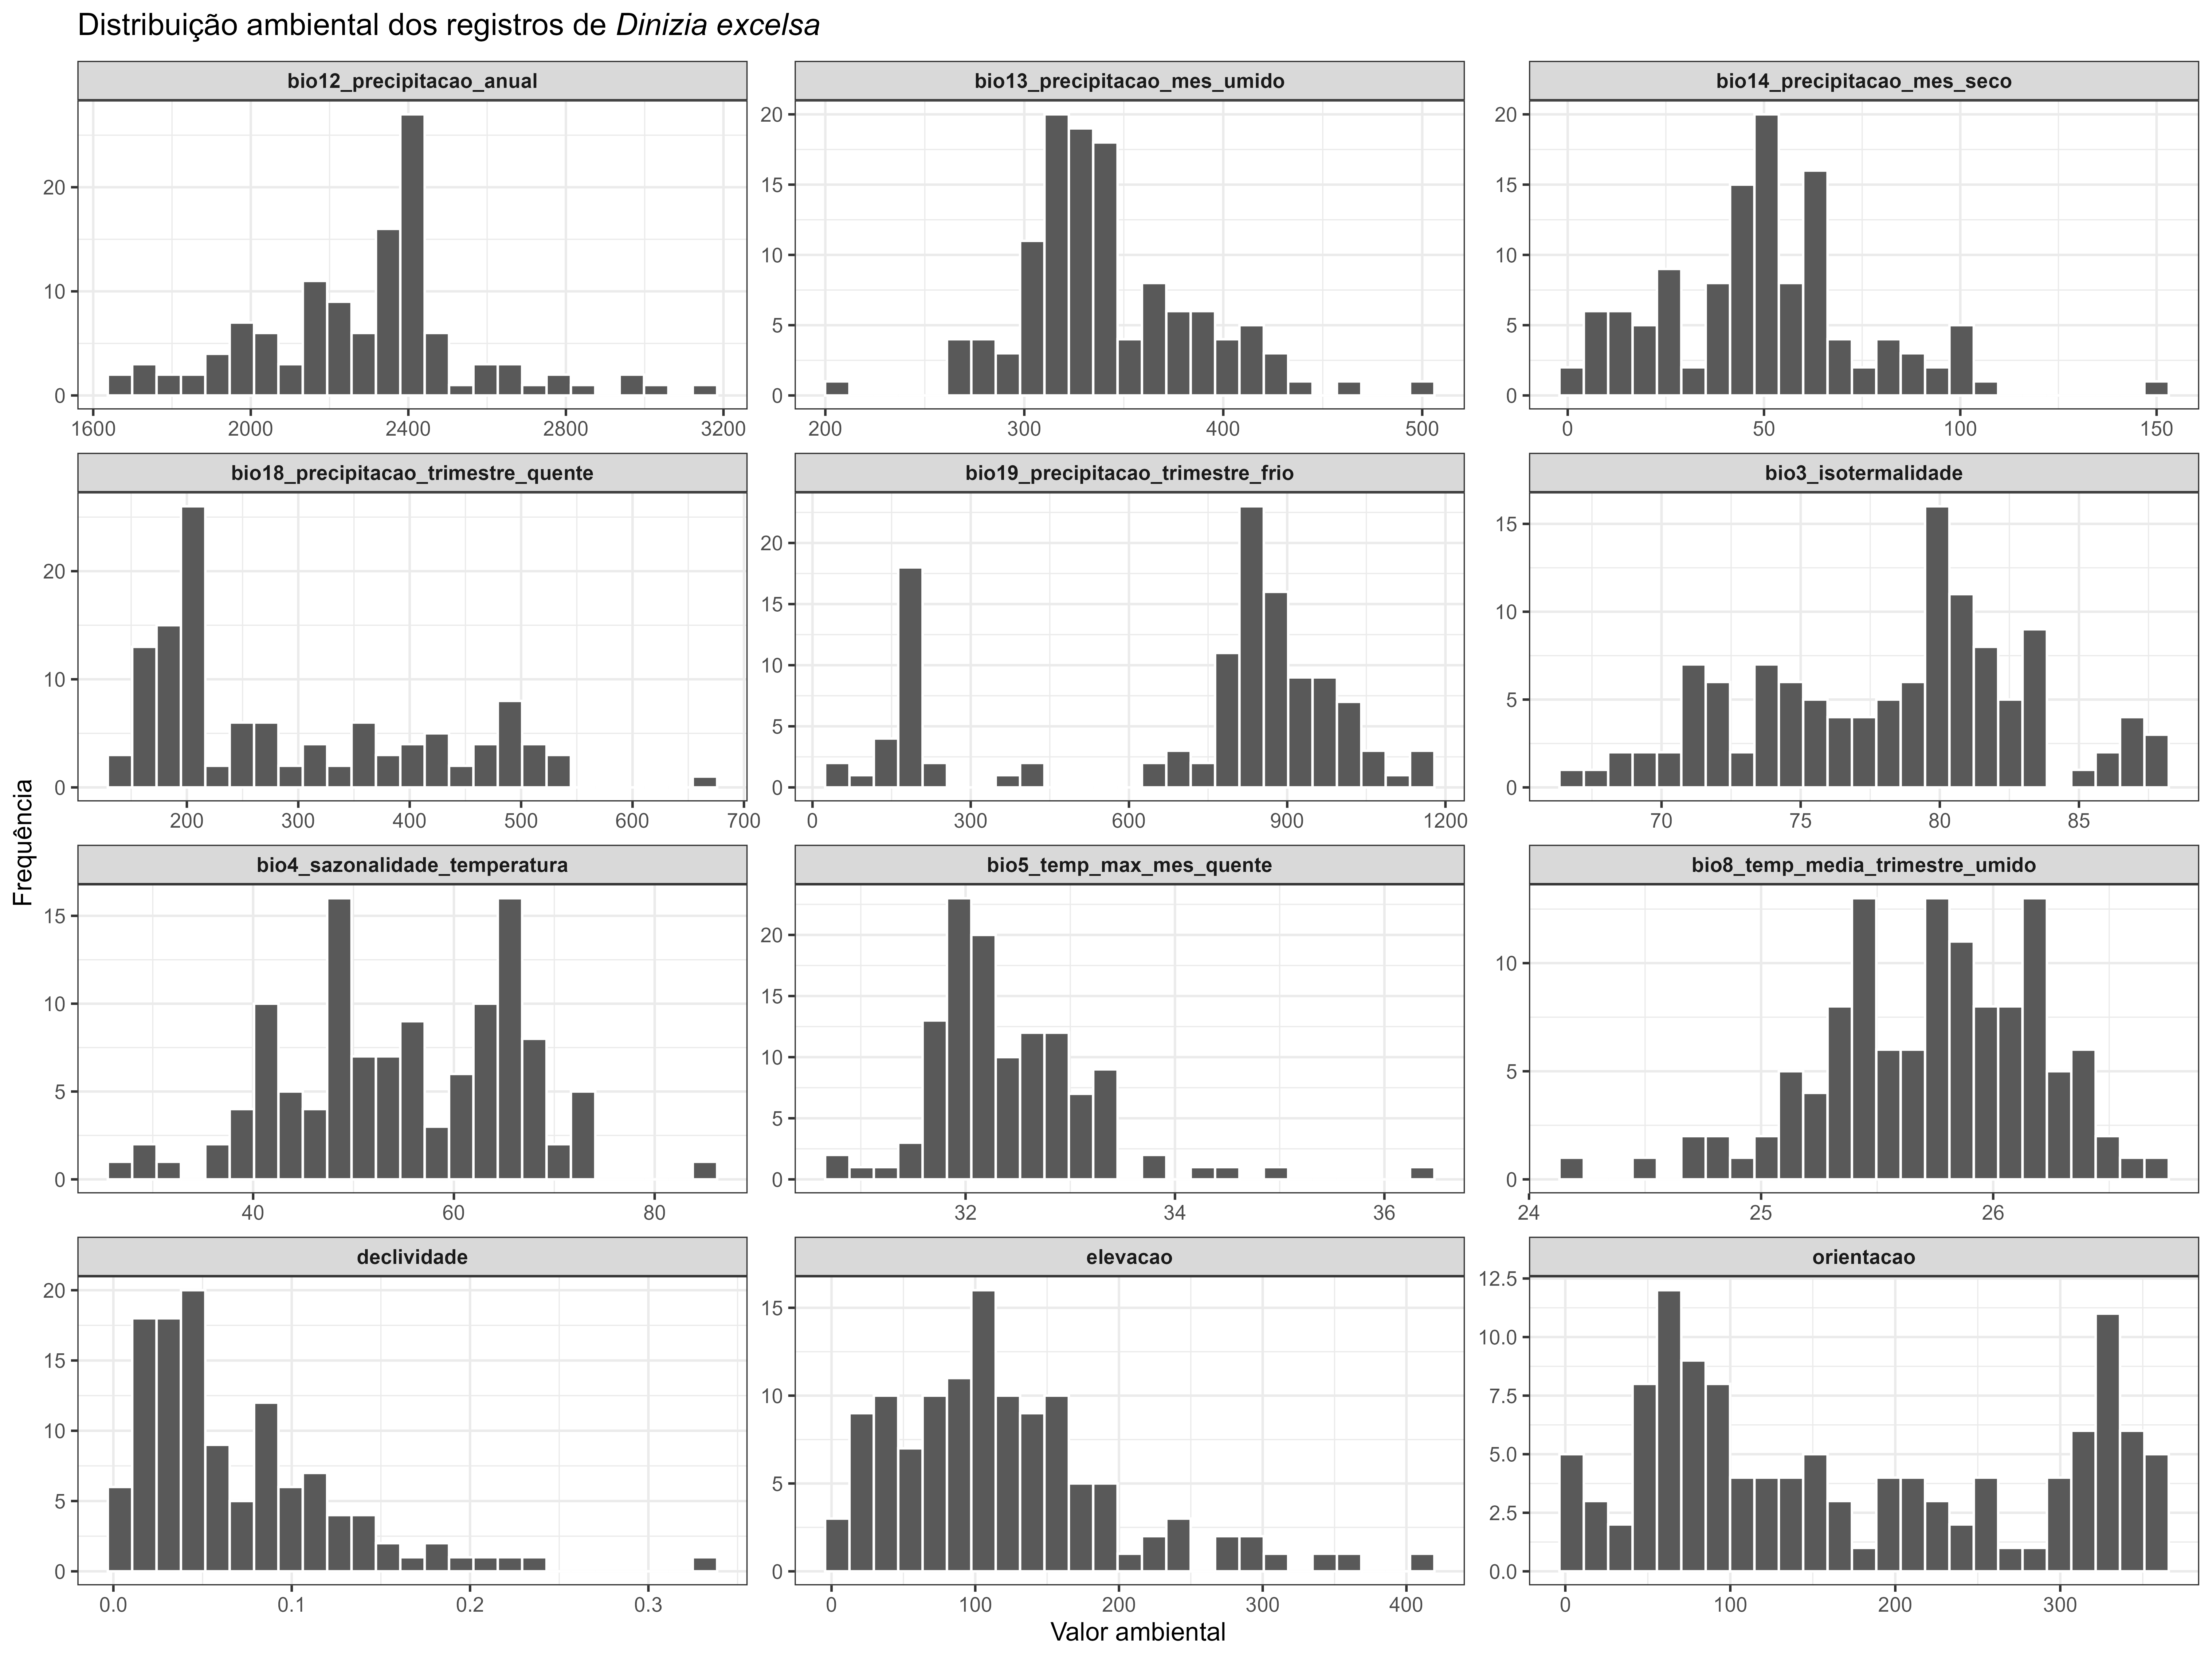
\includegraphics[width=0.94\textwidth]{figuras/unidade03/unidade03_histogramas_ambientais_dinizia.png}
	\caption{Distribuição das variáveis ambientais extraídas nos registros finais de \textit{Dinizia excelsa}. Os histogramas permitem avaliar a amplitude ambiental ocupada pela espécie em relação às variáveis selecionadas.}
	\label{fig:unidade03_histogramas_dinizia}
\end{figure}

\section{Produtos gerados pela Unidade 3}

O script desta unidade gera os seguintes produtos principais:

\begin{itemize}
	\item raster multivariado com variáveis bioclimáticas selecionadas para o bioma Amazônia;
	\item raster com variáveis topográficas harmonizadas;
	\item pilha ambiental completa para uso nas próximas unidades;
	\item tabela com valores ambientais extraídos nas ocorrências de \textit{Dinizia excelsa};
	\item background ambiental do bioma Amazônia;
	\item metadados das camadas ambientais;
	\item mapas bioclimáticos, mapas topográficos e histogramas ambientais.
\end{itemize}

\begin{dica}[title={\faLightbulb\quad Organização dos arquivos}]
	Os arquivos gerados nesta unidade devem ser mantidos como referência para as unidades seguintes. A pilha ambiental salva em \texttt{dados/unidade03/processados/variaveis\_ambientais\_amazonia\_unidade03.tif} será utilizada em análises de multicolinearidade, seleção de variáveis, modelagem e projeções.
\end{dica}

\section{Síntese da unidade}

As variáveis ambientais representam a ponte entre o nicho ecológico e a modelagem espacial. A seleção adequada dessas variáveis exige conhecimento ecológico, coerência com a escala da pergunta, compatibilidade com os registros de ocorrência e cuidado técnico no processamento espacial. Bases como WorldClim, CHELSA, EarthEnv, ENVIREM, SoilGrids e SRTM são extremamente úteis, mas devem ser usadas criticamente.

No estudo de caso com \textit{Dinizia excelsa}, a preparação das camadas ambientais para o bioma Amazônia permitiu construir uma base espacial reprodutível para as próximas etapas da apostila. A partir deste ponto, os dados já estão organizados para avaliar multicolinearidade, selecionar variáveis, ajustar modelos e produzir mapas de adequabilidade atual, passada e futura.

\begin{conceito}[title={\faBook\quad Mensagem central}]
	Em SDM, variáveis ambientais não são apenas camadas de mapa. Elas representam hipóteses ecológicas sobre os fatores que limitam, favorecem ou estruturam a distribuição das espécies.
\end{conceito}

\section{Exercícios de fixação}

\begin{enumerate}
	\item Explique a diferença entre espaço geográfico e espaço ambiental.
	\item Por que uma variável ambiental importante no modelo não representa necessariamente um mecanismo ecológico causal?
	\item Diferencie resolução espacial, extensão geográfica e escala ecológica.
	\item Explique por que variáveis climáticas são amplamente usadas em SDM de ampla escala.
	\item Cite exemplos de variáveis topográficas importantes para distribuição de espécies.
	\item Explique a importância de variáveis edáficas em modelos de distribuição de plantas.
	\item Por que é necessário harmonizar camadas ambientais antes da modelagem?
	\item No estudo de caso com \textit{Dinizia excelsa}, quais variáveis ambientais poderiam representar disponibilidade hídrica?
	\item Por que os rasters precisam ter a mesma resolução, extensão e CRS antes da modelagem?
\end{enumerate}

% ============================================================
% UNIDADE 4
% ============================================================

